\chapter{Physics Objects Reconstruction}
\section{Track and vertex reconstruction}
\label{sec:track}
Track and vertex reconstruction is a starting point of physics objects reconstruction, 
which make it crucial to understand how tracks and vertices are reconstructed in ATLAS.
Track reconstruction~\cite{ATLAS-CONF-2012-042,PERF-2015-08} is done 
mainly with the ``inside-outside'' procedure, complemented by the ``outside-in'' 
and the reconstructing of TRT-standalone tracks. 
% As shown in Figure~\ref{fig:electron_recon}, a charged particle traverses
% the ID. Space points are formed using the ID information.

The inside-out stage starts from assembling clusters from the raw measurements.
An algorithm called connected component analysis \cite{CCA} 
groups pixels and strips in a given sensor, 
where the deposited energy yields a charge above threshold, 
with a common edge or corner into clusters. 
It is useful to introduce the several classes of clusters identified 
by either the ``truth information'' (remove if this is mentioned earlier), 
only available in simulation and referring to information at MC generator level, 
or reconstructed quantities in both collision data and MC simulation. 
Clusters created by charge deposits from one particle
are called \textit{single-particle} clusters. Clusters created by charge
deposits from multiple particles are called \textit{merged} clusters.
These definitions rely on truth information and both cases
are illustrated in Figure \ref{fig:cluster}. 
In addition, clusters that are used in multiple reconstructed tracks 
but are not sufficiently compatible with the properties of a merged cluster
to be identified as merged by the reconstruction are called \textit{shared} clusters.
 \begin{figure}[bth]
    \centering
    \begin{subfigure}[t]{.38\linewidth}
        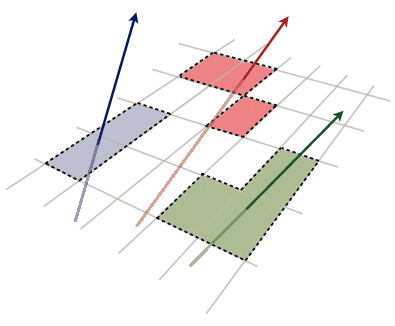
\includegraphics[width=1\textwidth]{Reconstruction_plots/single_cluster.png}
        \caption{(a)}
    \end{subfigure}
    \begin{subfigure}[t]{.38\linewidth}
        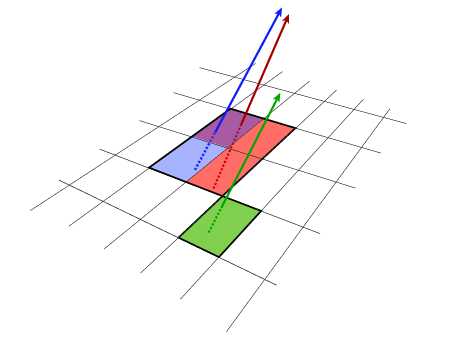
\includegraphics[width=1\textwidth]{Reconstruction_plots/merged_cluster.png}
        \caption{(b)}
    \end{subfigure}
    
    \caption{Illustration of (a) single-particle pixel clusters on a pixel sensor and (b) 
    a merged pixel cluster due to very collimated charged particles. 
    Different colours represent energy deposits from different charged particles 
    traversing the sensor and the particles trajectories are shown as arrows. 
    Image taken from \cite{PERF-2015-08}.}
    \label{fig:cluster}
\end{figure}
From clusters, three-dimensional measurements referred to as
\textit{space points} are created (the yellow points in Figure~\ref{fig:track_recon}). 
They represent the point where the charged particle 
traversed the active material of the ID. 
Each space point equates to one cluster in the pixel detector, while in the SCT, 
clusters from both sides of a strip layer must be combined to obtain a three-dimensional measurement.
Once the space points are created, three sets of space points are combined to track seeds 
(circled in blue in \ref{fig:track_recon}). 
This approach maximizes the possible number of combinations while still allowing 
a first crude momentum estimate. The impact parameters of a track seed, 
with respect to the centre of the interaction region, are estimated by assuming 
a perfect helical trajectory in a uniform magnetic field.
A combinatorial Kalman filter~\cite{FRUHWIRTH1987444} is used to 
build track candidates from the chosen seeds by incorporating additional 
space points from the remaining layers of the pixel and SCT detectors which 
are compatible with the preliminary trajectory. 
\begin{figure}[bht]
    \begin{centering}	
    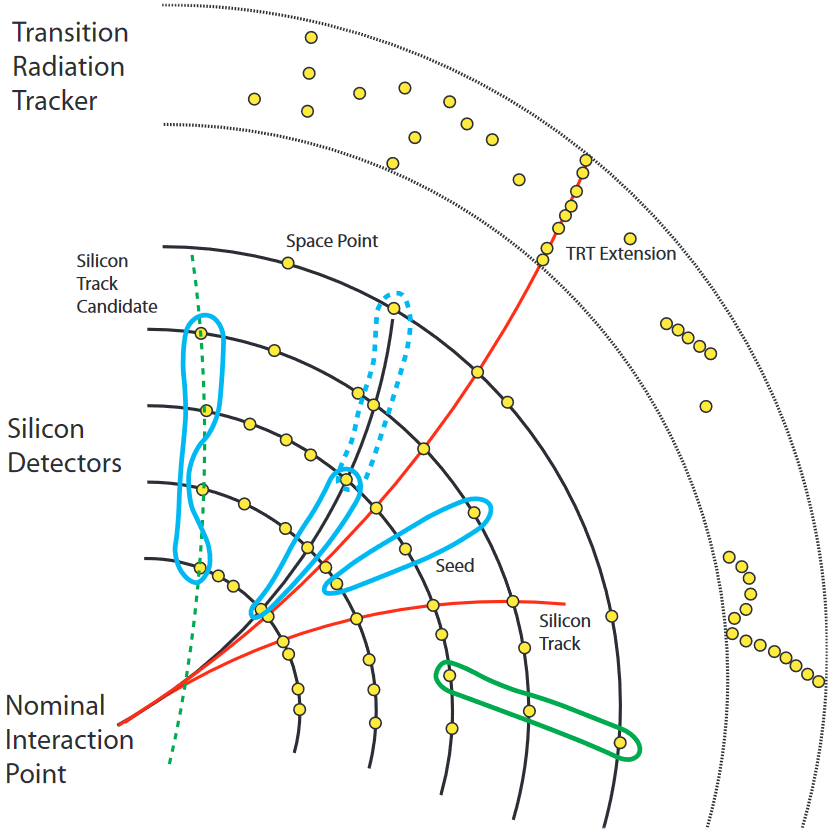
\includegraphics[width=.8\textwidth]{Reconstruction_plots/track.png}
    \caption{An example of track reconstruction. Image take from~\cite{ATLAS-CONF-2010-072}.
        }
    \label{fig:track_recon}
    \end{centering}
\end{figure}
A track score is assigned to each track,
which is computed by the $\chi^2$ of fitting the track, intrinsic resolution, 
expected clusters multiplicity, number of holes (missing hits) and track \pt. 
The tracks candidates are processed in descending order of 
track score. Track candidates fulfilling additional requirement 
on \pt\, number of holes, number of clusters etc. are fitted;
fitted tracks which pass through the selection without further modification
are added to the final track collection; tracks with too many shared clusters 
(with additional artificial neural network to identify them) are striped down and re-scored, 
and returned to the ordered list of remaining candidates. 
Finally, the tracks are extended into the TRT, and by using the full information
of the three sub-detectors, the tracks are fitted again to estimate the final track
impact parameter (IP, transverse distance from the interaction point) $d_0$, 
distance from the interaction point along the $z$ axis $z_0$,
azimuthal angle $\phi$, polar angle $\theta$ and charge momentum ratio $q/p_T$.
The complementary ``outside-in'' algorithm starts with searching for tracks with segments 
reconstructed in the TRT, and extend the tracks inwards by adding silicon hits. 
Back-tracking is designed to reconstruct tracks of secondary particles, which are
produced in the interactions of primary particles.
Finally, tracks with a TRT segment but no extension into the silicon detectors
are referred as TRT-standalone tracks. 

After the tracks are reconstructed, primary vertices reconstruction is done in two steps~\cite{ATLAS-CONF-2010-069}:
a) the primary vertex finding algorithm, dedicated to associate reconstructed tracks to the vertex candidates, 
and b) the vertex fitting algorithm, dedicated to reconstruct the vertex position. 
Vertex seeds are obtained from the $z$-position at the beamline of the reconstructed tracks. 
An iterative $\chi^2$ fit is made using the seed and nearby tracks. 
Each track carries a weight which is a measure of its compatibility 
with the fitted vertex depending on the $\chi^2$ of the fit. 
Vertices are required to contain at least two tracks, and 
tracks displaced by more than 7$\sigma$ from the vertex are used to
seed a new vertex and the procedure is repeated until no additional vertices can be found. 
This procedure is repeated until no unassociated tracks are left in the event or no
additional vertex can be found. 




\section{Electron}

\subsection{Electron reconstruction}
An electron can lose a significant amount of its energy through bremsstrahlung when traversing the detector,  
where the radiated photon can convert into an electron–positron pair which itself can
interact with the detector material. These positrons, electrons, and photons are usually very
collimated are normally reconstructed as part of the same electromagnetic cluster. 
These interactions can occur inside the inner-detector volume or even in the beam pipe, generating multiple tracks
in the inner detector, or can instead occur downstream of the inner detector, only impacting the shower in
the calorimeter. Therefore, it is possible to produce and match multiple tracks to the same electromagnetic
cluster, all originating from the same primary electron.

The reconstruction of electron is based on three fundamental components: 
a) localised clusters of energy deposits found within the EM calorimeter, 
b) charged tracks identified in the ID (as described in details in chapter~\ref{sec:track}),
and c) close matching in $\eta \times \phi$ space of the tracks to the clusters~\cite{PERF-2017-01}.
Figure~\ref{fig:electron_recon} provides a schematic illustration of the elements that enter into
the reconstruction and identification of an electron. 
\begin{figure}[bht]
    \begin{centering}	
    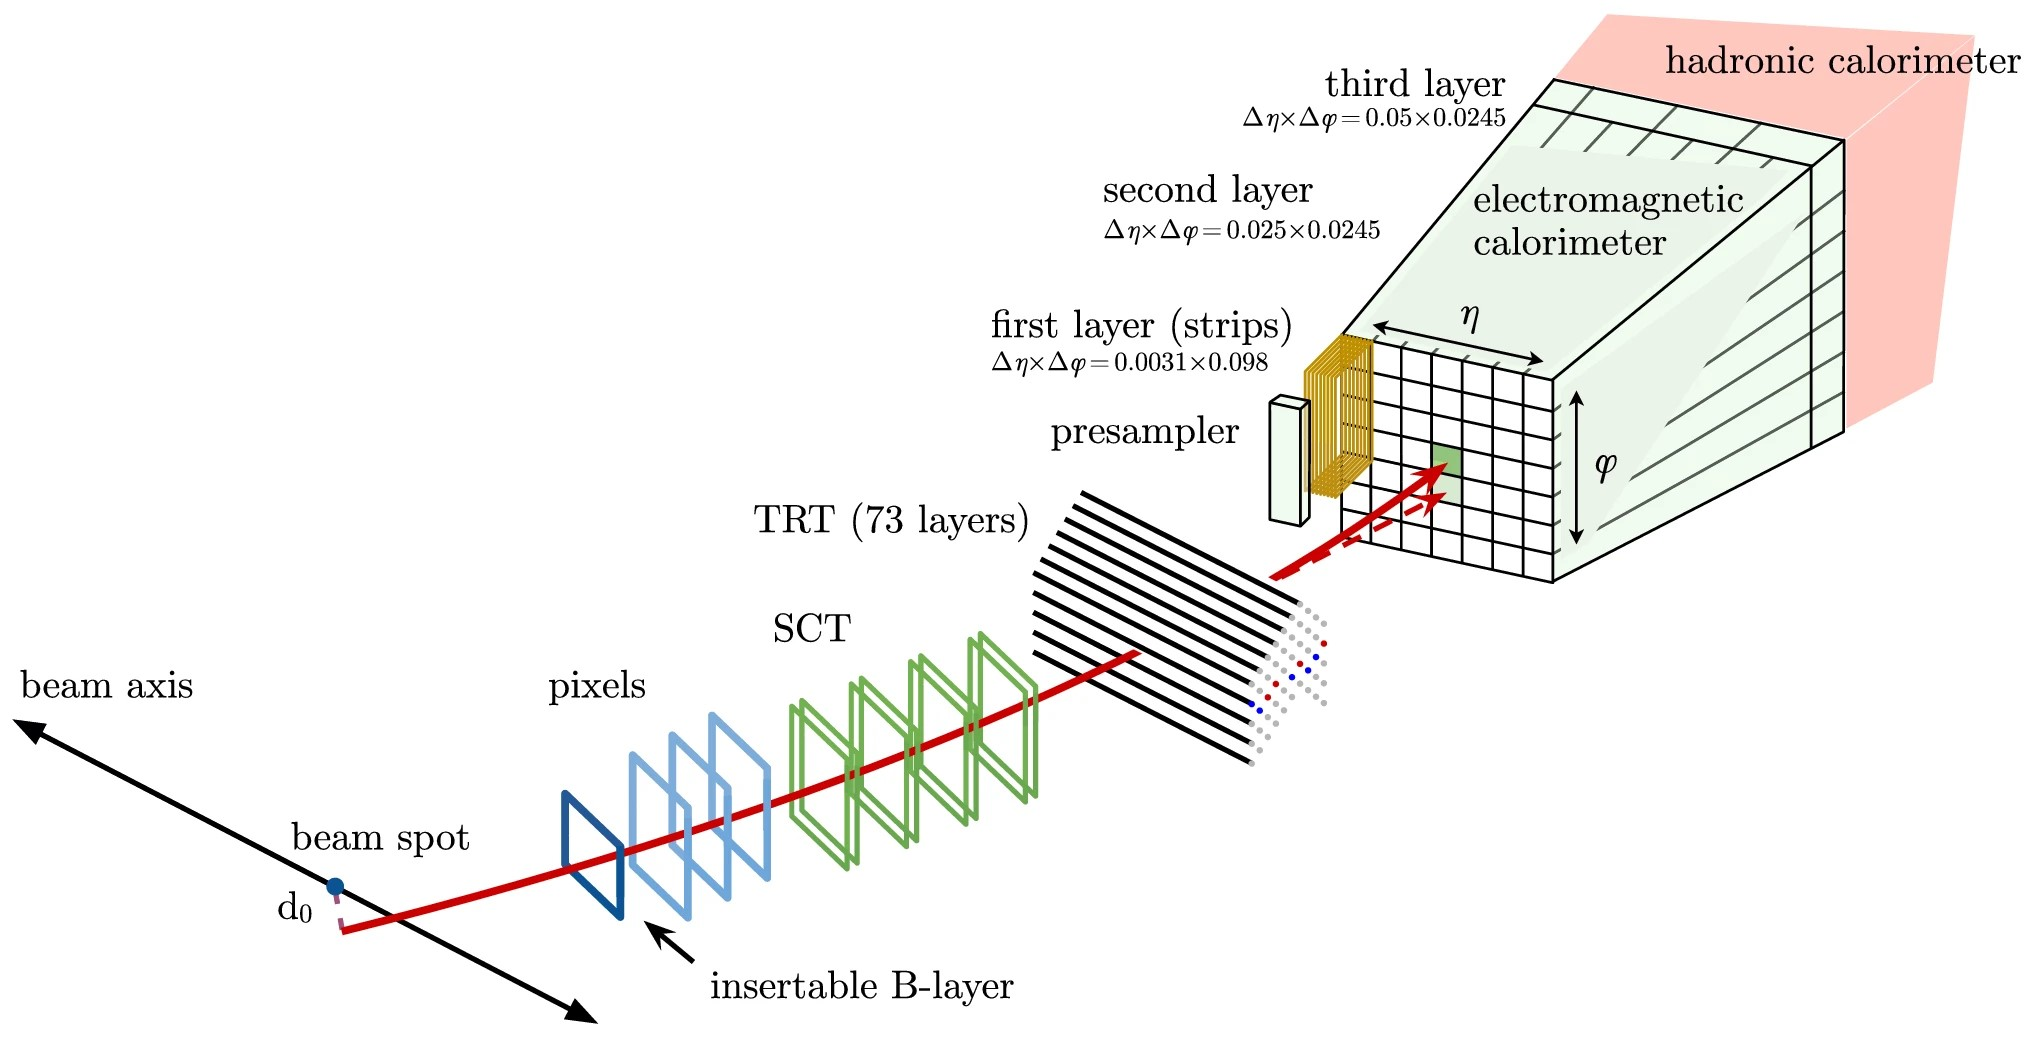
\includegraphics[width=.8\textwidth]{Reconstruction_plots/electron.jpg}
    \caption{A schematic illustration of the path of an electron through the detector. 
    The red trajectory shows the 
    hypothetical path of an electron, which first traverses the tracking system (pixel detectors, then SCT
    and lastly the TRT) and then enters the electromagnetic calorimeter. 
    The dashed red trajectory indicates the path of a
    photon produced by the interaction of the electron with the material in the tracking system. 
    Image taken from~\cite{PERF-2017-01}.
        }
    \label{fig:electron_recon}
    \end{centering}
\end{figure}

The reconstruction starts from EM cluster seeding from localised energy deposits 
using a sliding-window algorithm~\cite{sliding-window}.
The $\eta \times \phi$ space of the EM is divided into \textit{towers} of 200 $\times$ 256
elements of size $\Delta\eta \times \Delta\phi$ = 0.025 $\times$ 0.025, consistent with the
granularity of the second layer of the EM calorimeter. Then algorithm then ``slides'' a rectangular
window of size 3 $\times$ 5 towers whose summed transverse energy exceeds 2.5 GeV to form a seed-cluster.
The centre of the seed moves in steps of 0.025 in either $\eta$ or $\phi$ direction to search for localised
energy deposits; this process is repeated until every element of the calorimeter has been covered.
To better account for the energy loss of charged particles in material, a subsequentl fitting procedure
using optimised Gaussian-sum filter \cite{ATLAS-CONF-2012-047} is performed on tracks which are loosely 
matched to the EM clusters. The matching of the fitted tracks to the candidate calorimeter seed-cluster
is the final step of electron reconstruction. 
The matching requires $-0.10 < \Delta\phi \equiv -q \times (\phi_{cluster} - \phi_{track}) < 0.05$, 
where $q$ is the sign of charge of the particle, $\phi_{cluster}$ and $phi_{track}$ are the 
$\phi$ coordinates of the cluster barycentre and the poisition of the track extrapolated from the 
perigee to the second layer of the calorimeter, respectively. 
If several tracks fulfil the matching criteria, the track considered to
be the primary electron track is selected using an algorithm that takes into account the distance in $\eta$
and $\phi$ between the extrapolated tracks and the cluster barycentres (agian, measured in the second layer of the
calorimeter), 
the number of hits in the silicon detectors, 
and the number of hits in the innermost silicon layer; 
a candidate with an associated track with at least four hits in the silicon layers and no association
with a vertex from a photon conversion is considered as an electron candidate. 
However, if the primary candidate track can be matched to a secondary vertex and has no pixel hits, 
then this object is classified as a photon candidate (likely a conversion). 
A further classification is performed using the candidate electron’s $E/p$ and \pt, 
the presence of a pixel hit, and the secondary-vertex information, to determine
unambiguously whether the object is only to be considered as an electron candidate or if it should be
ambiguously classified as potentially either a photon candidate or an electron candidate.

\subsection{Electron identification}
Electron built by the reconstruction are not necessarily prompt electrons,
i.e. electrons coming from the collision of the an event; other objects, 
for example hadronic jets or non-prompt electrons,
may produce a signature which is reconstructed as an electron. 
Therefore, a likelihood technique is employed to select prompt electrons ~\cite{PERF-2017-01}.
The inputs to the likelihood include measurements from the tracking system, the
calorimeter system, and quantities that combine both tracking and calorimeter information.
The main advantages using the likelihood-based method comparing with 
a selection-criteria-based (so-called ``cut-based'') identification is that
a prompt electron may fail the cut-based identification because it
does not satisfy the selection criterion for a single quantity, 
while in the likelihood-based selection this electron can
still satisfy the identification criteria, 
because the likelihood combines the information of all of the discriminating variables.
The final discriminant produced by the likelihood method is used to define 
three \textit{working points}, which are cuts in the final discriminant 
identifying the different identification efficiencies. The working points are
\textit{Loose}, \textit{Medium} and \textit{Tight}. 
TODO: Find electron identification and isolation working points for bbtautau and Ftag

\section{Muon}



\section{Muon}
\section{Jet}
